% %%%%%%%%%%%%%%%%%%%%%%%%%% Figure 1 Oversiktskart %%%%%%%%%%%%%%%%%%%%%%%%%%%%
\begin{figure}[t]
 \setlength{\unitlength}{1.0cm}
 \begin{center}
  \begin{pspicture}(0,0)(15,11)
% Include graphs
   \rput[b](7.5,0){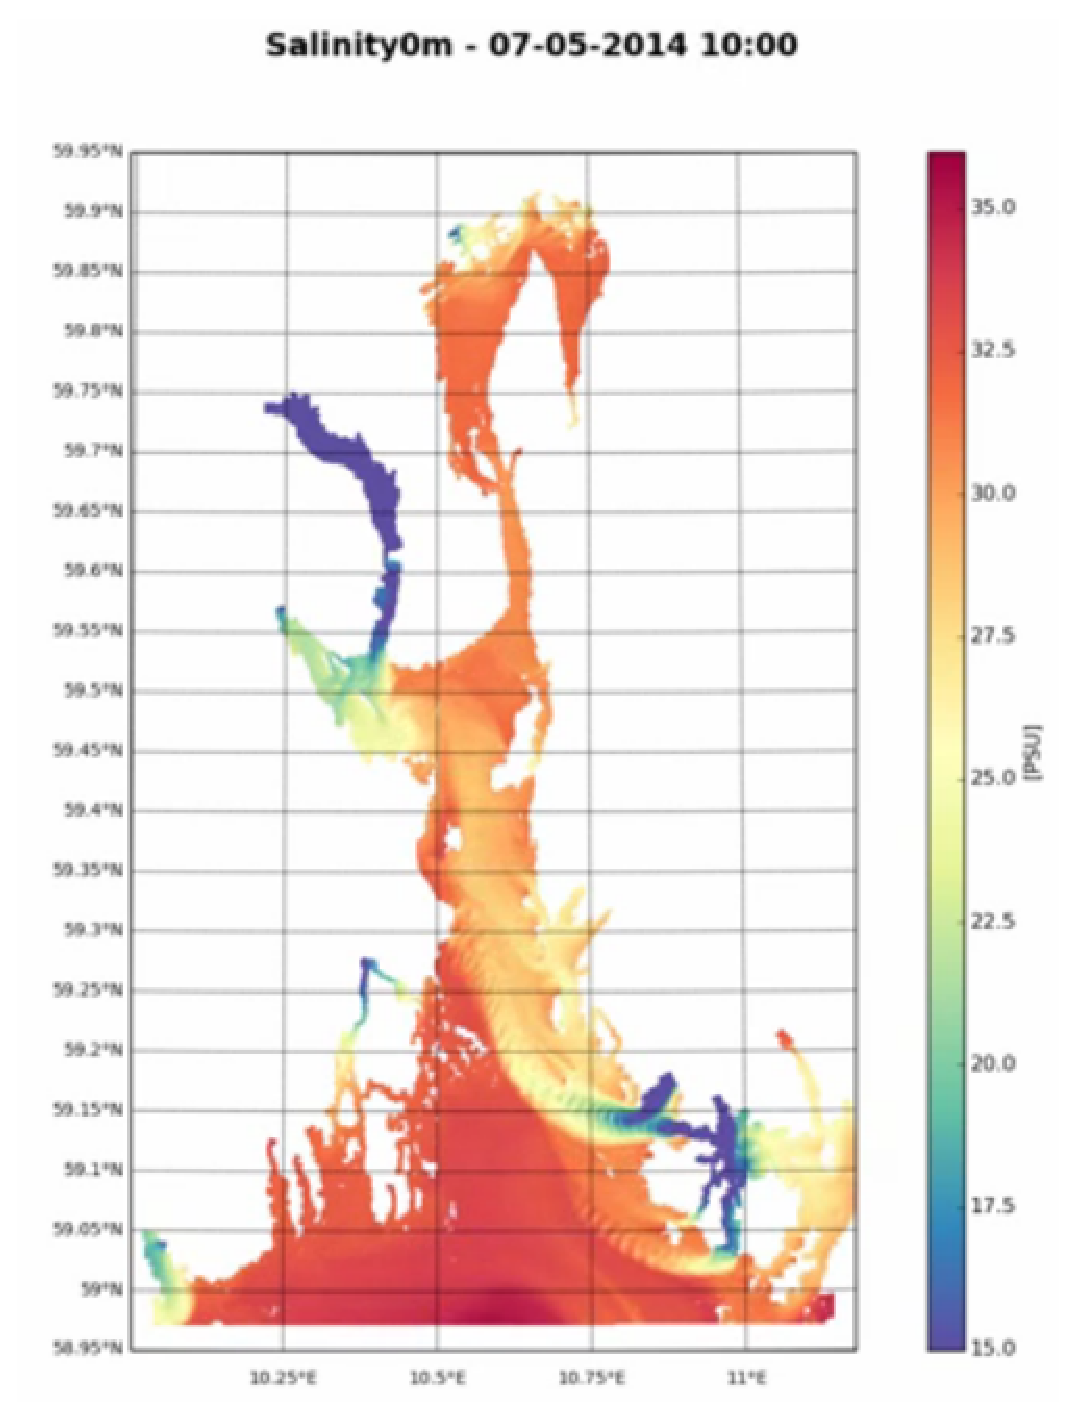
\includegraphics[height=11cm]{FjordOs_salinity_2014-05-07_14UTC}}
  \end{pspicture}
% Figure caption is below the figure
  \caption{Sea surface salinity at 10:00 UTC on May 5, 2014. Colorbar indicates salinity in the range 15 (blue) to 35 (red) psu. Note the impact of the freshwater discharge from the major rivers Glomma (located in the southeast) and Dramselva (located to the northwest), and also the many minor rivers.}   \label{fig:mainmap}       % Give a unique label
 \end{center}
\end{figure}
%

